\colorbox{white!10!}{
    \begin{minipage}{0.2\textwidth}
       \begin{flushleft}
        \includegraphics[width = 0.6\textwidth]{Эмблема.png}
       \end{flushleft}
    \end{minipage}
    \begin{minipage}[t]{0.7 \textwidth}
        \begin{center}
            {\huge \textsc{Красноярская Летняя Школа. Сезон $7^2 - 2$}}
            \vspace{0.25cm}
            
            { \huge \textbf{ФМТ. Тур 3.1}}
        \end{center}
        \vspace{0.05cm}
    \end{minipage}
}

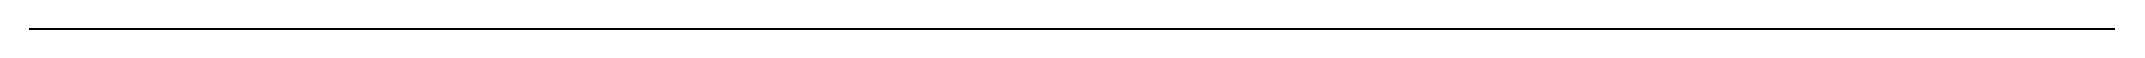
\begin{tikzpicture}
    \draw[thick] (-6.5,0)--(20,0);
\end{tikzpicture}
\begin{enumerate}
    \parbox[b]{.7\textwidth}{%
    \item На рисунке изображена конструкция из: палки массой $M$, двумя отдельными нитями и груза массы $m$ (см. рис) 
    Определите силу натяжения нити AB. Угол $\alpha$ считать известным.
    }\hfill\includegraphics[width=.145\textwidth]{pictures/Tur_3.png}
	
 
    \item Два зеркала образуют двугранный угол $\varphi$. На одно из них падает под углом $\alpha$ луч, перпендикулярный ребру угла. На какой угол отклонится этот луч после двух отражений?
\end{enumerate}